\section{Results}\label{sec:results}
We first confirm that the starting point is sound, then report the label-free comparison,
then test why it comes out as it does.

\subsection{The reproduction holds}
On the authors' released inputs and under their own protocol, MICA reaches the published
ARI within 0.05 on nine of ten datasets and within 0.001 on six. The exception is
Kolodziejczyk, where the released files give 0.727 against a published 1.000, and the
authors' own notebook also gives 0.727, so the published value appears to come from an
input that was not released. These numbers were established in Assignment 2 and are
unchanged. They matter here only because they license the comparison that follows: when
the labels fix the setting, our MICA runs behave as the paper reports.

\begin{table}[t]
\centering
\caption{ARI of the partition the stability rule chose under each of its two readings, with the number of clusters chosen in parentheses and the true number of cell types after each dataset name. No reference labels are used in the choice. Values are medians over three seeds, and a pair such as (15-18) gives the smallest and largest count over those seeds. The mean row covers the nine small-data datasets, the set every mean in the text refers to. PBMC14K runs in MICA's graph mode and is discussed in Section~\ref{sec:pbmc}. The other two rules are in Table~\ref{tab:rulesall}, and Table~\ref{tab:common} gives this rule on the cluster counts the baseline produces.}
\label{tab:rules}
\footnotesize
\setlength{\tabcolsep}{4pt}
\resizebox{\columnwidth}{!}{%
\begin{tabular}{lcccc}
\toprule
 & \multicolumn{2}{c}{Finest stable} & \multicolumn{2}{c}{Most stable} \\
\cmidrule(lr){2-3}\cmidrule(lr){4-5}
Dataset (types) & MICA & Leiden & MICA & Leiden \\
\midrule
Yan (8) & 0.496\,(19\textrm{-}20) & 0.845\,(5\textrm{-}8) & 0.496\,(3) & 0.765\,(4\textrm{-}5) \\
Goolam (5) & 0.593\,(6\textrm{-}7) & 0.429\,(2\textrm{-}3) & 0.630\,(2\textrm{-}3) & 0.619\,(2\textrm{-}3) \\
Buettner (3) & 0.934\,(3) & 0.232\,(3) & 0.474\,(2\textrm{-}3) & 0.134\,(2\textrm{-}3) \\
Pollen (11) & 0.898\,(15\textrm{-}18) & 0.755\,(7\textrm{-}11) & 0.087\,(2) & 0.755\,(5\textrm{-}11) \\
Chung (4) & 0.474\,(11\textrm{-}12) & 0.129\,(3\textrm{-}4) & 0.100\,(2) & 0.129\,(3) \\
Usoskin (4) & 0.818\,(3) & 0.633\,(6) & 0.818\,(3) & 0.757\,(3\textrm{-}6) \\
Kolodziejczyk (3) & 0.722\,(3\textrm{-}5) & 0.838\,(4) & 0.630\,(2) & 0.838\,(4) \\
Klein (4) & 0.501\,(2\textrm{-}3) & 0.973\,(4) & 0.501\,(2) & 0.859\,(3\textrm{-}4) \\
Zeisel (7) & 0.518\,(3) & 0.855\,(8\textrm{-}9) & 0.518\,(2\textrm{-}3) & 0.855\,(8) \\
PBMC14K (7) & 0.629\,(5) & 0.397\,(4) & 0.629\,(5) & 0.397\,(4) \\
\midrule
\textit{Mean, nine small} & \textbf{0.661} & \textbf{0.632} & \textbf{0.473} & \textbf{0.635} \\
\bottomrule
\end{tabular}
}
\end{table}


\subsection{The ranking depends on the selection rule, not on the data}
Table~\ref{tab:rules} reports what each method achieves when the same rule chooses its
setting without labels. The two stability columns are the same scores read two ways. The
published chooseR rule keeps the finest setting that clears a reproducibility threshold.
The second column keeps the highest-scoring setting outright.

Under the published reading, MICA leads on five of eight datasets with a mean ARI of 0.675
against 0.595. Under the second reading, MICA leads on three of eight with a mean of 0.467
against 0.583. The ranking reverses. The two columns use identical subsamples, identical
candidate settings and identical scores, and differ only in how settings that score alike
are separated.

The size of the movement is the result. Between the two readings MICA's mean ARI changes by
0.208, while the baseline's changes by 0.012. The baseline is nearly indifferent to the
tie-break and MICA is not, which is why a single rule reported alone would look like a
statement about the two methods when it is partly a statement about the rule.

Individual datasets show the same pattern more sharply. On Pollen MICA scores 0.896 under
the published reading and 0.087 under the other, because the first keeps 18 clusters and the
second collapses to 2. Neither is close to the 11 types actually present.

\begin{table}[t]
\centering
\caption{Number of clusters each rule chose. The true number of types is in brackets after the dataset name. A rule can reach a fair ARI with a badly wrong cluster count, which a user would notice.}
\label{tab:clusters}
\scriptsize
\setlength{\tabcolsep}{3pt}
\begin{tabular}{lcccc}
\toprule
 & \multicolumn{2}{c}{Finest stable} & \multicolumn{2}{c}{Most stable} \\
\cmidrule(lr){2-3}\cmidrule(lr){4-5}
Dataset (types) & MICA & Leiden & MICA & Leiden \\
\midrule
Yan (8) & n/a & n/a & n/a & n/a & 19 & 8 & 3 & 5 \\
Goolam (5) & n/a & n/a & n/a & n/a & 6 & 3 & 2 & 2 \\
Buettner (3) & n/a & n/a & n/a & n/a & 3 & 3 & 2 & 3 \\
Pollen (11) & n/a & n/a & n/a & n/a & 18 & 7 & 2 & 5 \\
Chung (4) & n/a & n/a & n/a & n/a & 12 & 3 & 2 & 3 \\
Usoskin (4) & n/a & n/a & n/a & n/a & 3 & 6 & 3 & 6 \\
Kolodziejczyk (3) & n/a & n/a & n/a & n/a & 3 & 4 & 2 & 4 \\
\bottomrule
\end{tabular}
\end{table}


\subsection{The chosen cluster counts}
Table~\ref{tab:clusters} shows why the ARI values alone understate the problem. Under the
published reading MICA chooses 19 clusters on Yan, which has 8 types, 18 on Pollen, which
has 11, and 12 on Chung, which has 4. A user inspecting those partitions would see the
problem at once, which is the argument for reporting the count next to the score. The
baseline's counts are closer to the truth on most datasets, and where it fails it fails by
merging rather than by splitting.

\begin{figure*}[t]
\centering
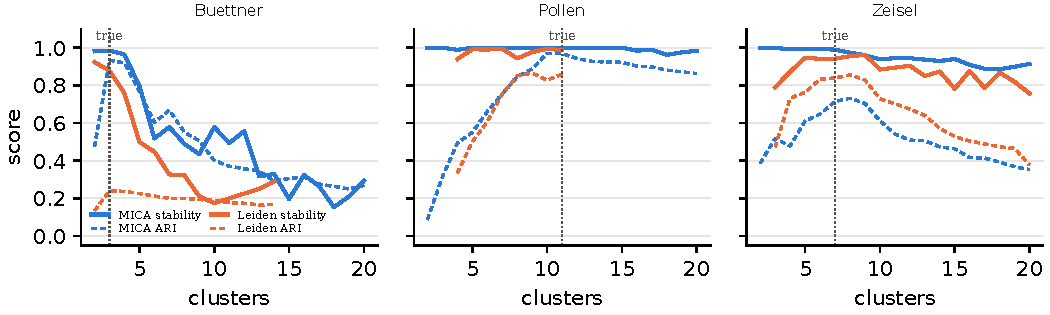
\includegraphics[width=\textwidth]{figures/a3_stability_curve.pdf}
\caption{Reproducibility and accuracy against the number of clusters, for both methods on
three datasets. Solid lines are the stability score the rule maximises, dashed lines the
ARI against the reference labels, and the dotted vertical line marks the true number of
types. Where the solid line is flat, the rule has no basis for preferring one setting over
another and its tie-break decides instead.}
\label{fig:curve}
\end{figure*}

\subsection{Why: the rule cannot separate the settings}
Figure~\ref{fig:curve} shows the quantity the rule maximises, plotted against the number of
clusters. On Buettner MICA's stability falls steadily as clusters are added, the rule has a
clear maximum near the true value, and it selects 3 clusters for an ARI of 0.934. On Pollen
MICA's stability stays close to its maximum across the whole range from 2 to 20 clusters,
so there is nothing for the threshold to discriminate on.

Measured across all datasets, 38 percent of MICA's candidate settings score within 0.01 of
its best, against 27 percent for the baseline. The consequence is clearer in cluster counts
than in scores: among the settings that tie with the best, the span of cluster counts
averages 6.9 for MICA and 2.5 for the baseline. On Yan the rule cannot separate 3 clusters
from 19.

This explains the reversal. When many settings tie, the rule's preference decides, and the
published rule prefers the finest. It also yields a prediction we can test: the worse the
ambiguity, the worse the overclustering should be. Across datasets the association between
the spread of a method's stability scores and the excess over the true cluster count has a
Spearman correlation of $-0.74$ for MICA and $-0.24$ for the baseline, in the predicted
direction and much stronger for the method whose scores are compressed. With eight
datasets this is a consistency check rather than a test, and we report it as such.

One explanation we expected does not hold. We supposed that stability would simply carry
less information about accuracy for MICA. It carries slightly more: the rank correlation
between stability and ARI across settings averages 0.69 for MICA against 0.50 for the
baseline. The problem is not that the signal points the wrong way but that it is compressed
into a band too narrow for a threshold to act on.

\subsection{Cost}
The rule costs 494 clusterings per dataset for MICA over 19 candidate values of $k$, and
about 1,040 for the baseline over its resolution grid, in both cases 25 subsample reruns
plus the full-data fit. On the datasets here that is 15 to 92 seconds for MICA and 14 to
211 seconds for the baseline on 8 threads, excluding the mutual information distance
matrix, which is computed once per dataset and shared by every setting and seed.

That one-off cost is the larger number and it falls only on MICA: 6 to 11 minutes on the
two datasets above 2,500 cells, against seconds on the smallest. It is also what makes the
rule affordable at all. Because MICA's distance between two cells does not depend on any
other cell, the matrix is computed once and subsampled exactly, rather than recomputed 25
times. Without that property the rule would cost roughly 25 times more for MICA, and the
comparison in Table~\ref{tab:rules} would not have been feasible on this hardware.
